\begin{figure}[htbp]
\centering
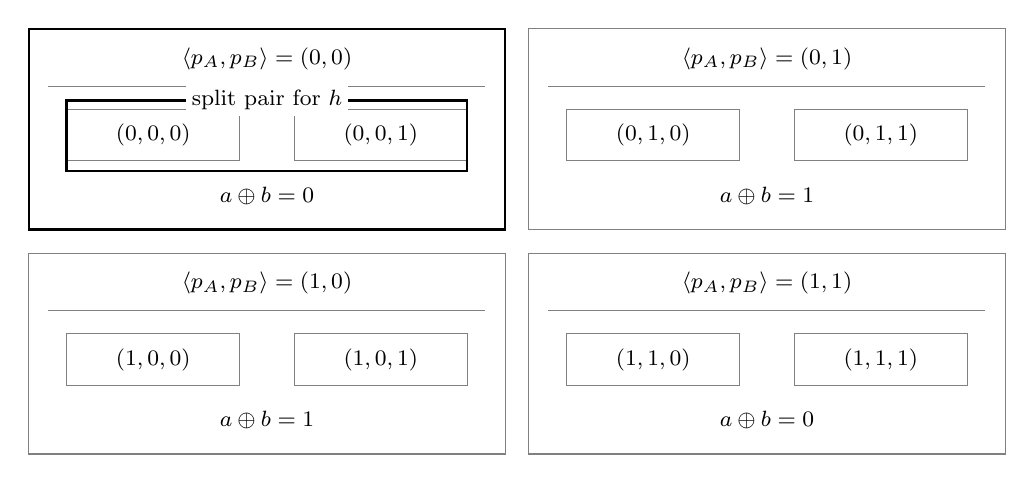
\begin{tikzpicture}[font=\footnotesize]
  \foreach \x/\y/\a/\b/\v in {
    0/0/0/0/0, 6.35/0/0/1/1,
    0/-2.85/1/0/1, 6.35/-2.85/1/1/0} {
    \draw[gray] (\x,\y) rectangle ++(6.05,-2.55);
    \node at (\x+3.025,\y-0.38)
      {$\langle p_A,p_B\rangle=(\a,\b)$};
    \draw[gray] (\x+0.25,\y-0.73) -- (\x+5.8,\y-0.73);
    \node[draw=gray,minimum width=2.2cm,minimum height=0.65cm]
      at (\x+1.58,\y-1.35) {$(\a,\b,0)$};
    \node[draw=gray,minimum width=2.2cm,minimum height=0.65cm]
      at (\x+4.47,\y-1.35) {$(\a,\b,1)$};
    \node at (\x+3.025,\y-2.12) {$a\oplus b=\v$};
  }
  \draw[black,thick] (0,0) rectangle (6.05,-2.55);
  \draw[black,thick] (0.48,-1.81) rectangle (5.57,-0.91);
  \node[fill=white,inner sep=2pt] at (3.025,-0.91) {split pair for $h$};
\end{tikzpicture}
\caption{The four fibres of $\langle p_A,p_B\rangle$ in $\{0,1\}^3$. Each contains both values of $h$ and one value of $a\oplus b$; the outlined states in the $(0,0)$ fibre form a split pair for $h$.}
\label{fig:cube}
\end{figure}
